\section{Implementasi}

\subsection{Basis Data}
\begin{figure}[H]
	\centering
		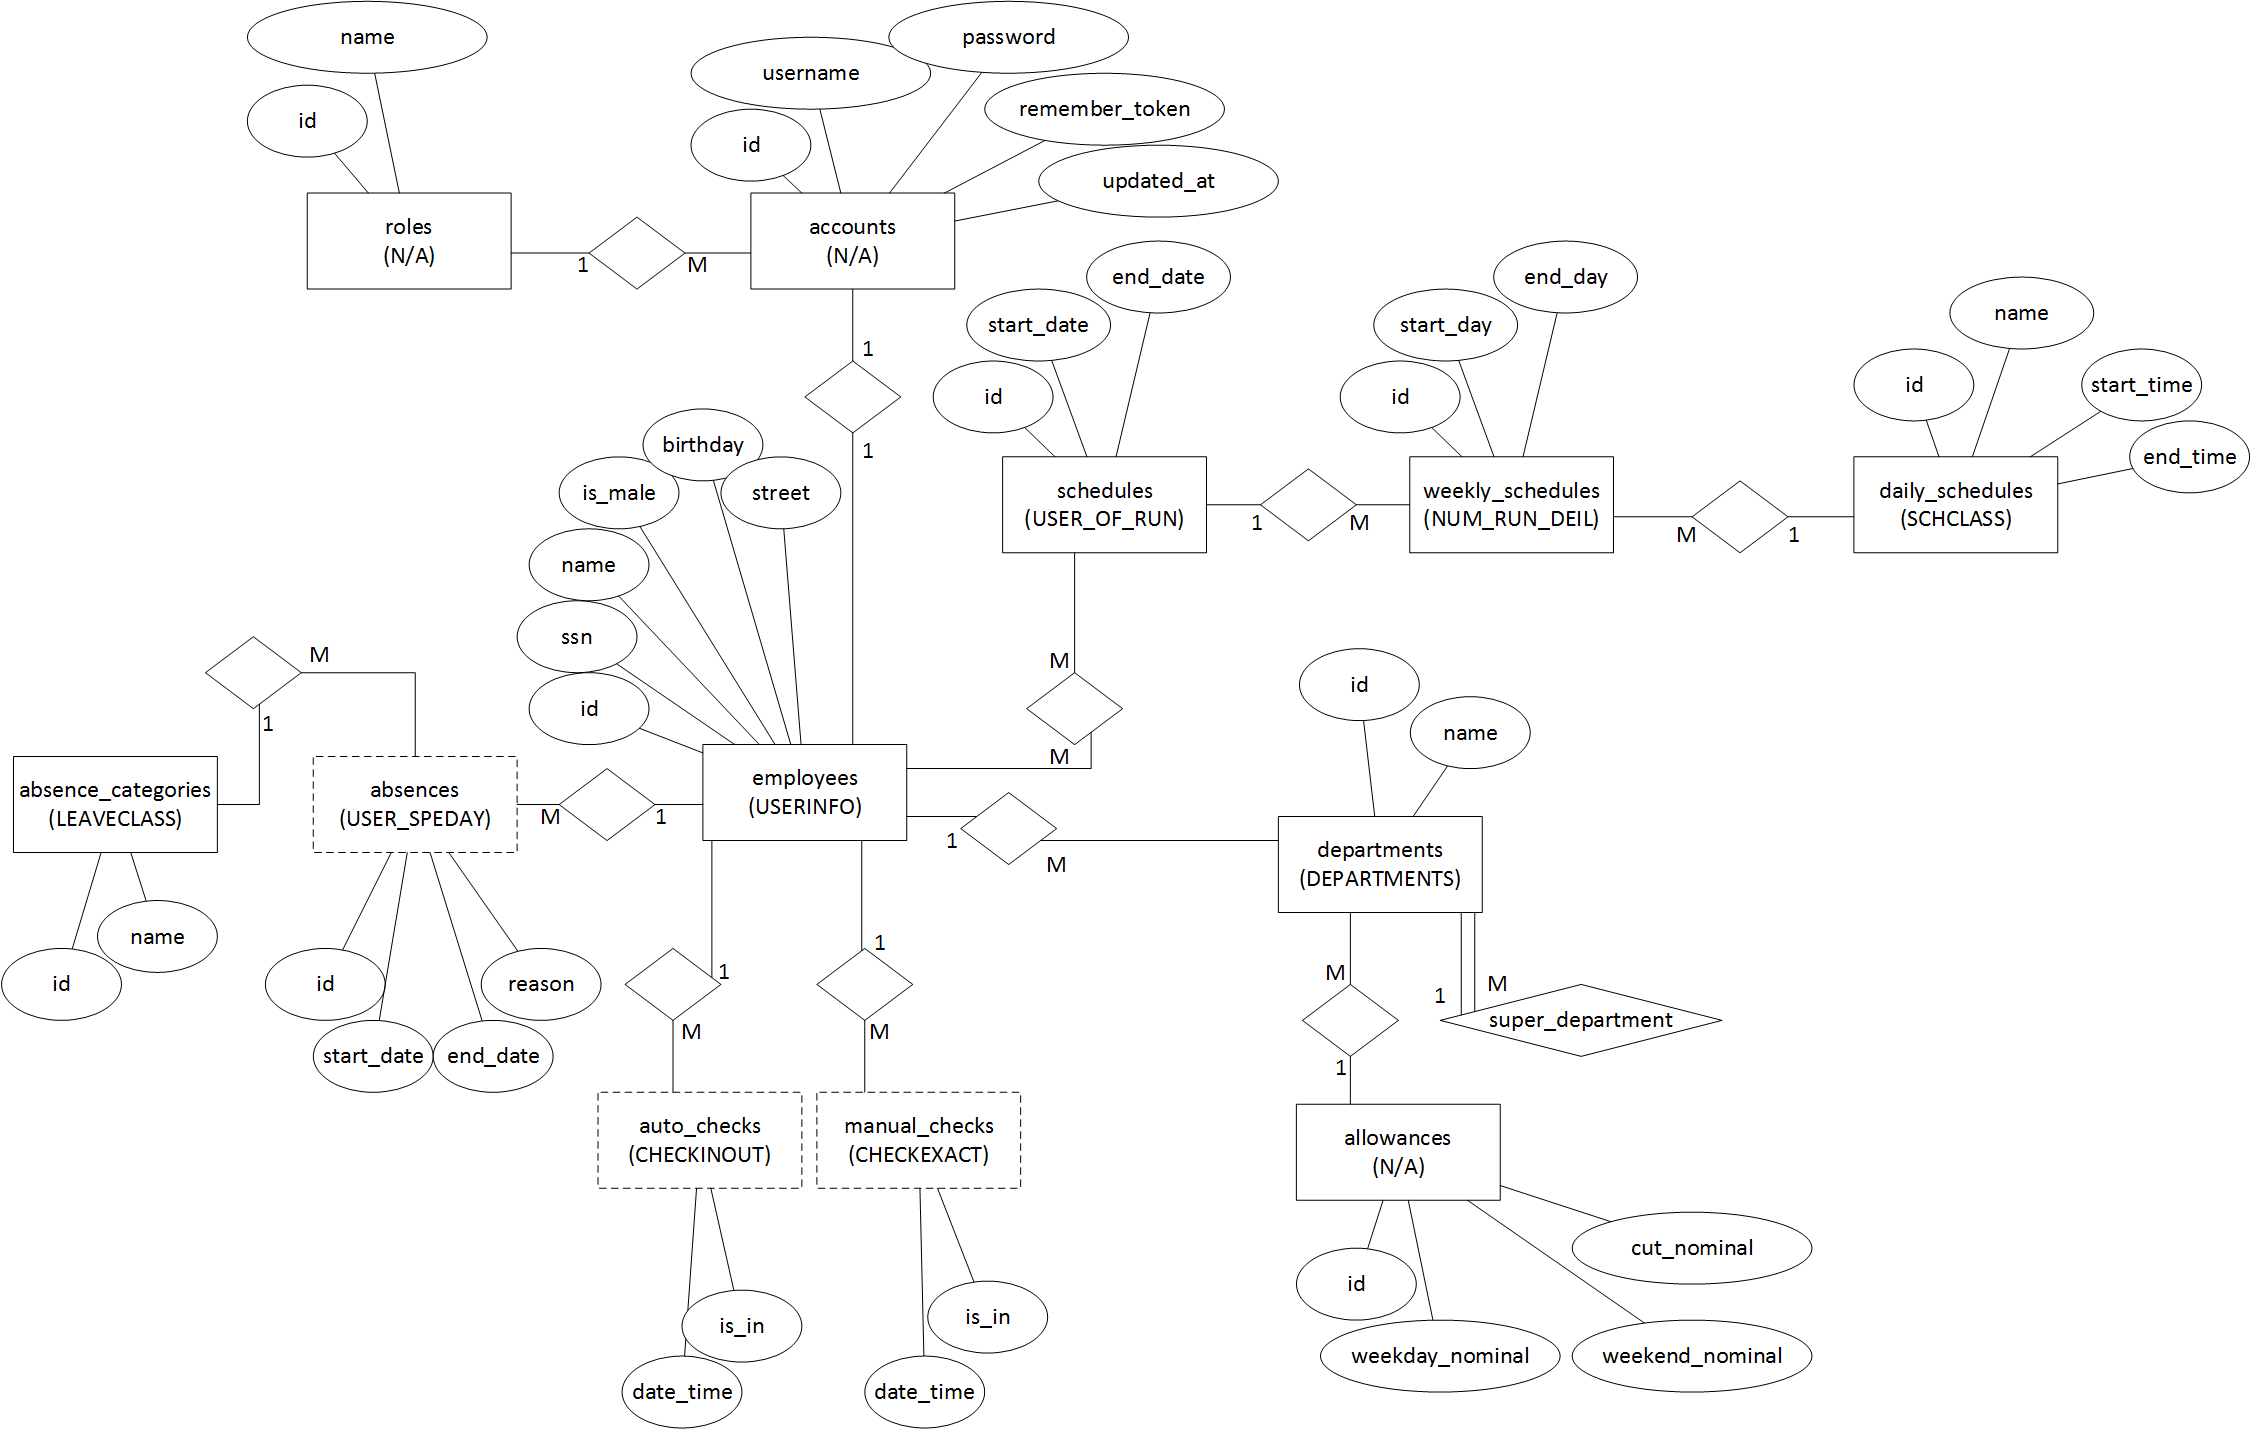
\includegraphics[width=1.00\textwidth]{gambar/erd.png}
	\caption{Diagram \textit{Entity Relationship}}
	\label{fig:erd}
\end{figure}

\subsection{Lingkungan Pendukung}
\begin{itemize}
	\item \textit{Framework}
\\Sistem informasi ini adalah sistem informasi berbasis web. Sistem informasi ini dibangun dengan \textit{framework} Laravel 4.2.\footnote{http://laravel.com/docs/4.2/quick} 
	\item Basis Data
\\Basis data yang digunakan selama proses pembangunan sistem ini adalah MySql. 
	\item \textit{Web Server} 
\\Basis data yang digunakan selama proses pembangunan sistem ini adalah Apache.
\end{itemize}

\pagebreak



